\documentclass{article}
\usepackage{graphicx}
\usepackage{amsmath,amssymb}
\usepackage{graphicx}
\usepackage{hyperref}
\usepackage{geometry}
\usepackage{enumitem}
\usepackage{times}
\usepackage{fancyhdr}
\usepackage{fontspec}
\usepackage{unicode-math}
\setmainfont{Times New Roman}
\setmathfont{Cambria Math}

\title{EAS PEMODELAN MATEMATIKA (C)}
\author{Pak Kamiran}
\date{}

\begin{document}

\fancyhead[L]{\textit{Teosofi Hidayah Agung}}
\fancyhead[R]{\textit{5002221132}}
\pagestyle{fancy}

\maketitle

\section*{Soal 1}

Perhatikan model dengan sistem persamaan diferensial serta kontrol $U_1(t)$ dan $U_2(t)$, sebagai berikut:
\[
\frac{dx}{dt}=(1-u_1)y^2-x^2 \quad \text{dan} \quad \frac{dy}{dt} = x-u_2xy
\]
Dengan syarat awal:
\[
x(0) = 1 \quad \text{dan}\quad y(0) = 2
\]
maka:

\begin{enumerate}[label=\alph*.]
    %nomor 1
    \item Tentukan titik stabilitas non-negatif dan linierkan model tersebut untuk nilai kontrol $u_1 = \frac{3}{4} \text{ dan } u_2=\frac{1}{2}$. \\
    \textbf{Jawab}: Titik stabilitas non negatif dari persamaan tesebut adalah saat $\frac{dx}{dt} = 0$ dan $\frac{dy}{dt} = 0$ serta nilai koordinat $(x,y)$ memiliki nilai non negatif. Maka
    \begin{align*}
        \frac{dx}{dt}=(1-u_1)y^2-x^2 &=0 \\
        (1-\frac{3}{4})y^2 &=x^2 \\
        \frac{y^2}{4}&=x^2
    \end{align*}
    Sehingga diperoleh persamaan \eqref{eq.1} sebagai berikut
    \begin{equation}
        y^2 =4x^2 \label{eq.1}
    \end{equation}
    Serta
    \begin{align*}
        \frac{dy}{dt} = x-u_2xy &=0 \\
        x-\frac{1}{2}xy &=0 \\
        x(1-\frac{1}{2}y)&=0\\
        x=0 \text{ atau}&\ y=2
    \end{align*}
    Subsitusi $x=0$ dan $y=2$ pada persamaan \eqref{eq.1}. Sehingga diperoleh saat $x=0$ maka $y=0$ dan saat $y=2$ maka diperoleh x sebagai berikut
    \begin{align*}
        4x^2 &=2^2 \\
        4x^2 &=4 \\
        x^2 &= 1 \\
        x &= \pm 1
    \end{align*}
    Oleh karena itu diperoleh 3 titik stabilitas yaitu $(0,0)$, $(1,2), \text{ dan } (-1,2)$, dengan titik stabilitas nonnegatif yaitu $\textbf{(1,2)}$ dan $\textbf{(0,0)}$. \\
    Selanjutnya akan dilakukan pelinieran model tersebut dengan menggunakan matriks Jacobian:
    \[
    J = 
    \begin{bmatrix}
    \frac{\partial}{\partial x}\left( \frac{dx}{dt} \right) & \frac{\partial}{\partial y}\left( \frac{dx}{dt} \right) \\
    \frac{\partial}{\partial x}\left( \frac{dy}{dt} \right) & \frac{\partial}{\partial y}\left( \frac{dy}{dt} \right)
    \end{bmatrix}_{(x^*,y^*)}
    \]
    Dengan $(x^*,y^*)$ adalah titik stabilitas yang didapat sebelumnya, maka matriks Jacobian adalah sebagai berikut
    \[
    J = 
    \begin{bmatrix}
    \frac{\partial}{\partial x}\left( (1-u_1)y^2-x^2 \right) & \frac{\partial}{\partial y}\left( (1-u_1)y^2-x^2 \right) \\
    \frac{\partial}{\partial x}\left( x-u_2xy \right) & \frac{\partial}{\partial y}\left( x-u_2xy \right)
    \end{bmatrix}_{(x^*,y^*)} =
    \begin{bmatrix}
    -2x & \frac{1}{2}y \\
    1-\frac{1}{2}y & -\frac{1}{2}x
    \end{bmatrix}_{(x^*,y^*)}
    \]
    Apabila menggunakan titik kesetimbangan $\textbf{(1,2)}$, maka matriks Jacobian menjadi
    \[
    J = 
    \begin{bmatrix}
    -2x & \frac{1}{2}y \\
    1-\frac{1}{2}y & -\frac{1}{2}x
    \end{bmatrix}_{(1,2)}
    = 
    \begin{bmatrix}
    -2(1) & \frac{1}{2}(2) \\
    1-\frac{1}{2}(2) & -\frac{1}{2}(1)
    \end{bmatrix}
    = 
    \begin{bmatrix}
    -2 & 1 \\
    0 & -\frac{1}{2}
    \end{bmatrix}
    \]
    Dan menggunakan titik kesetimbangan $\textbf{(0,0)}$, diperoleh matriks Jacobian sebagai berikut
    \[
    J = 
    \begin{bmatrix}
    -2x & \frac{1}{2}y \\
    1-\frac{1}{2}y & -\frac{1}{2}x
    \end{bmatrix}_{(0,0)}
    = 
    \begin{bmatrix}
    -2(0) & \frac{1}{2}(0) \\
    1-\frac{1}{2}(0) & -\frac{1}{2}(0)
    \end{bmatrix}
    = 
    \begin{bmatrix}
    0 & 0 \\
    1 & 0
    \end{bmatrix}.
    \]
    Sehingga setelah dilakukan pelinieran di sekitar titik kesetimbangan diperoleh 2 bentuk persamaan differensial yaitu
    \[
    \begin{bmatrix}
        \dot{x} \\ \dot{y}
    \end{bmatrix} =
    \begin{bmatrix}
    -2 & 1 \\ 0 & -\frac{1}{2}
    \end{bmatrix} 
    \begin{bmatrix}
        x \\ y
    \end{bmatrix} \quad \text{dan }
    \begin{bmatrix}
        \dot{x} \\ \dot{y}
    \end{bmatrix} =
    \begin{bmatrix}
    0 & 0 \\
    1 & 0
    \end{bmatrix} 
    \begin{bmatrix}
        x \\ y
    \end{bmatrix}
    \]

    
    %nomor 2
    \item Apakah model tersebut stabil dengan nilai kontrol tersebut? \\
    \textbf{Jawab}: Suatu sistem dikatakan stabil apabila nilai eigen model tersebut adalah negatif. Maka akan dihitung nilai eigen model dengan menggunakan persamaan:
    \[
    |A- \lambda I| = 0
    \]
    Dengan $A = \begin{bmatrix}
    -2 & 1 \\ 0 & -\frac{1}{2}
    \end{bmatrix}$ maka nilai eigennya adalah
    \begin{align*}
        \left| \begin{array}{cc}
    -2-\lambda & 1 \\
     0& -\frac{1}{2}-\lambda
    \end{array} \right| &= 0 \\
    (-2-\lambda)\left(-\frac{1}{2}-\lambda\right)&=0 \\
    \lambda_1=-2 \text{ dan } \lambda_2&=-\frac{1}{2}
    \end{align*}
    Karena kedua nilai eigen adalah negatif, maka model \textbf{stabil}. \\
    
    Untuk $A=\begin{bmatrix}
    0 & 0 \\
    1 & 0
    \end{bmatrix}$ maka nilai eigennya adalah
    \begin{align*}
        \left| \begin{array}{cc}
    -\lambda & 0 \\
     1& -\lambda
    \end{array} \right| &= 0 \\
    \lambda^2 &=0 \\
    \lambda_{1,2} &= 0
    \end{align*}
    Karena nilai eigen bernilai $0$, maka model \textbf{stabil tidak asimtotis}.

    %nomor 3
    \item Selesaikan bentuk linier dari sistem persamaan diferensial tersebut. \\
    \textbf{Jawab}: Akan dipilih model linier yang \textbf{stabil} dari sistem persamaan differensial yaitu 
    \[
    \begin{bmatrix}
        \dot{x} \\ \dot{y}
    \end{bmatrix} =
    \begin{bmatrix}
    -2 & 1 \\ 0 & -\frac{1}{2}
    \end{bmatrix} 
    \begin{bmatrix}
        x \\ y
    \end{bmatrix}
    \]
    Langkah pertama yaitu mencari nilai eigen yaitu didapat melalui perhitungan sebelumnya, nilai eigen sistem adalah $\lambda_1=-2$ dan $\lambda_2=-\frac{1}{2}$. 
    Selanjutnya mencari vektor eigen dengan persaman 
    \[ (A - \lambda I) \mathbf{v} = 0 \]
    \begin{itemize}
        \item Untuk $\lambda_1=-2$ diperoleh vektor eigen $v_1 = \begin{bmatrix}1 \\ 0\end{bmatrix}$
        \item Untuk $\lambda_2=-\frac{1}{2}$ diperoleh vektor eigen $v_2 = \begin{bmatrix}1 \\ \frac{3}{2}\end{bmatrix}$.
    \end{itemize}
    
    Sehingga penyelesaian umum sistem persamaan differensial yaitu
    \begin{align*}
        \begin{bmatrix}
            x \\ y
        \end{bmatrix} &= C_1e^{\lambda_1t}+C_2e^{\lambda_2t} \\
        \begin{bmatrix}
            x \\ y
        \end{bmatrix} &= C_1e^{-2t} \begin{bmatrix}
            1 \\ 0
        \end{bmatrix} + C_2e^{-\frac{1}{2}t}  \begin{bmatrix}
            1 \\ \frac{3}{2}
        \end{bmatrix}
    \end{align*}
    Kemudian akan dicari penyelesaian khusus sistem persamaan diferensial yaitu melalui nilai awal $x(0) = 1 \quad \text{dan}\quad y(0) = 2$.
    \begin{align*}
        \begin{bmatrix}
            x(0) \\ y(0)
        \end{bmatrix} &= C_1e^{-2 \times0} \begin{bmatrix}
            1 \\ 0
        \end{bmatrix} + C_2e^{-\frac{1}{2}\times 0}  \begin{bmatrix}
            1 \\ \frac{3}{2}
        \end{bmatrix} \\
        \begin{bmatrix}
            1 \\ 2
        \end{bmatrix} &= C_1 \begin{bmatrix}
            1 \\ 0
        \end{bmatrix} + C_2\begin{bmatrix}
            1 \\ \frac{3}{2}
        \end{bmatrix}
    \end{align*}
    Diperoleh
    \begin{align*}
        \frac{3}{2}C_2&=2\\
        C_2&=\frac{4}{3}
    \end{align*}
    dan \begin{align*}
        C_1+C_2&=1\\
        C_1&=1-\frac{4}{3} \\
        C_1 &= -\frac{1}{3}
    \end{align*}
    Sehingga penyelesaian khusus sistem persaman diferensial adalah
    \begin{align*}
        \begin{bmatrix}
            x \\ y
        \end{bmatrix} &= -\frac{1}{3}e^{-2t} \begin{bmatrix}
            1 \\ 0
        \end{bmatrix} + \frac{4}{3}e^{-\frac{1}{2}t}  \begin{bmatrix}
            1 \\ \frac{3}{2}
        \end{bmatrix}
    \end{align*}

    %nomor 4
    \item Selesaikan bentuk nonlinier dari sistem persamaan diferensial tersebut secara numerik (metode Runge-Kutta). \\
    \textbf{Jawab}: Rumus Runge-Kutta untuk menghitung iterasi $x_n$ dan $y_n$ adalah sebagai berikut:
    \[
    x_n = x_{n-1} + \frac{h}{6}(k_1 + 2k_2 + 2k_3 + k_4),
    \]
    \[
    y_n = y_{n-1} + \frac{h}{6}(l_1 + 2l_2 + 2l_3 + l_4).
    \]
    dengan:
    \[
    k_1 = h \cdot f(x_0, y_0), \quad l_1 = h \cdot g(x_0, y_0),
    \]
    \[
    k_2 = h \cdot f\left(x_0 + \frac{1}{2}k_1, y_0 + \frac{1}{2}l_1\right), \quad l_2 = h \cdot g\left(x_0 + \frac{1}{2}k_1, y_0 + \frac{1}{2}l_1\right),
    \]
    \[
    k_3 = h \cdot f\left(x_0 + \frac{1}{2}k_2, y_0 + \frac{1}{2}l_2\right), \quad l_3 = h \cdot g\left(x_0 + \frac{1}{2}k_2, y_0 + \frac{1}{2}l_2\right),
    \]
    \[
    k_4 = h \cdot f(x_0 + k_3, y_0 + l_3), \quad l_4 = h \cdot g(x_0 + k_3, y_0 + l_3).
    \]
    Hitung nilai $k$ dan $l$ yaitu
    \[
    k_1 = h \cdot f(x_0, y_0) = 0.1 \cdot \left(\left(1 - \frac{3}{4}\right)(2)^2 - (1)^2\right) = 0,
    \]
    \[
    l_1 = h \cdot g(x_0, y_0) = 0.1 \cdot \left(1 - \frac{1}{2}(1)(2)\right) = 0.
    \] \\
    \[
    k_2 = h \cdot f\left(x_0 + \frac{1}{2}k_1, y_0 + \frac{1}{2}l_1\right) = 0.1 \cdot f(1, 2) = 0,
    \]
    \[
    l_2 = h \cdot g\left(x_0 + \frac{1}{2}k_1, y_0 + \frac{1}{2}l_1\right) = 0.1 \cdot g(1, 2) = 0.
    \] \\
    \[
    k_3 = h \cdot f\left(x_0 + \frac{1}{2}k_2, y_0 + \frac{1}{2}l_2\right) = 0.1 \cdot f(1, 2) = 0,
    \]
    \[
    l_3 = h \cdot g\left(x_0 + \frac{1}{2}k_2, y_0 + \frac{1}{2}l_2\right) = 0.1 \cdot g(1, 2) = 0.
    \] \\
    \[
    k_4 = h \cdot f(x_0 + k_3, y_0 + l_3) = 0.1 \cdot f(1, 2) = 0,
    \]
    \[
    l_4 = h \cdot g(x_0 + k_3, y_0 + l_3) = 0.1 \cdot g(1, 2) = 0.
    \]
    Sehingga $x_1$ dan $y_1$ adalah 
    \[
    x_1 = x_0 + \frac{1}{6}(k_1 + 2k_2 + 2k_3 + k_4) = 1 + \frac{1}{6}(0 + 2(0) + 2(0) + 0) = 1,
    \]
    \[
    y_1 = y_0 + \frac{1}{6}(l_1 + 2l_2 + 2l_3 + l_4) = 2 + \frac{1}{6}(0 + 2(0) + 2(0) + 0) = 2.
    \]
    Karena iterasi yang cukup panjang maka untuk $x_n$ dan $y_n$ selanjutnya akan dilanjutkan dengan bantuan bahasa pemograman dalam bentuk grafik yang ada pada jawaban (e).
    
    %nomor 5
    \item Tampilkan grafik penyelesaian poin (c) dan (d) dalam satu frame. \\
    \textbf{Jawab}: Dengan menggunakan bantuan \textit{software} MATLAB, didapatkan grafik dibawah ini:
    
    \begin{figure}[h!] 
      \centering
      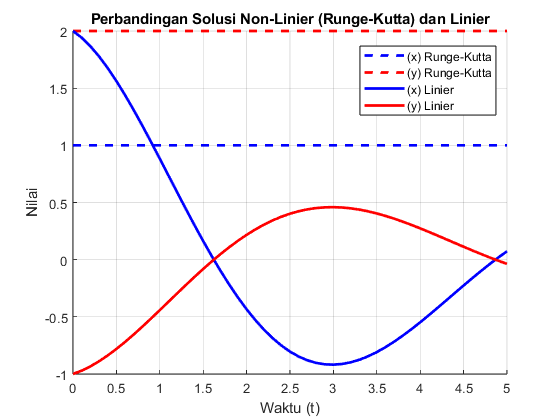
\includegraphics[width=0.7\linewidth]{EAS Nomor 1.png}
      \label{fig:simulasi2}
    \end{figure}
    
\end{enumerate}


\pagebreak
\section*{Soal 2}

Perhatikan model dengan sistem persamaan diferensial serta kontrol $U_1(t)$ dan $U_2(t)$, sebagai berikut:
\[
\frac{dx}{dt}=(1-u_1)y^2-x^2 \quad \text{dan} \quad \frac{dy}{dt} = x-u_2xy
\]
Dengan syarat awal:
\[
x(0) = 1 \quad \text{dan}\quad y(0) = 2
\]
Dan diberikan kontrol optimum sebagai berikut:
\[
J = \min \int_{0}^{10} \left(x+y+\frac{1}{2}(u_1^2+u_2^2)\right) dt
\]
Dengan; $0 \leq u_1 \leq 1 $, $0 \leq u_2 \leq 1$ memenuhi persamaan diferensial di atas.

\begin{enumerate}[label=\alph*.]
    %bagian a
    \item Nyatakan bentuk fungsi Hamiltonian dari model di atas.\\
    \textbf{Jawab}: Fungsi Hamiltonian yaitu
    \begin{align*}
        H(x,y,u_1,u_2,\lambda_1,\lambda_2) &= L(x,y,u_1,u_2)+\lambda_1\frac{dx}{dy} + \lambda_2\frac{dy}{dt} \\
        H(x,y,u_1,u_2,\lambda_1,\lambda_2) &= x+y+\frac{1}{2}(u_1^2+u_2^2) +\lambda_1\{(1-u_1)y^2-x^2\}+\lambda_2(x-u_2xy) \\
        H(x,y,u_1,u_2,\lambda_1,\lambda_2) &= x+y+\frac{1}{2}u_1^2+\frac{1}{2}u_2^2+\lambda_1y^2-\lambda_1u_1y^2-\lambda_1 x^2 + \lambda_2x - \lambda_2u_2xy
    \end{align*}
    Turunan parsial terhadap \(u_1\) dan \(u_2\) :
    \[
    \frac{\partial H}{\partial u_1}=u_1-\lambda_1y^2=0 \implies u_1 = \lambda_1 y^2
    \]
    \[
    \frac{\partial H}{\partial u_2}=u_2-\lambda_2xy=0 \implies u_1 = \lambda_2 xy
    \]
    
    %bagian b
    \item Linierkan model tersebut dan analisa kestabilannya pada titik stabilitas nonnegatif.\\
    \textbf{Jawab}: Titik stabilitas non negatif dari persamaan tesebut adalah saat $\frac{dx}{dt} = 0$ dan $\frac{dy}{dt} = 0$ serta nilai koordinat $(x,y)$ memiliki nilai non negatif. Maka
    \begin{align*}
        \frac{dx}{dt} &=0 \\
        (1-u_1)y^2-x^2 &=0 \\
        (1-u_1)y^2 &=x^2 \\
    \end{align*}
    Sehingga diperoleh
    \begin{equation}
        x=\pm \sqrt{1-u_1}y \label{eq.2}
    \end{equation}
    Selanjutnya pada
    \begin{align*}
        \frac{dy}{dt} &=0 \\
        x-u_2xy &=0 \\
        x(1-u_2y) &=0
    \end{align*}
    Diperoleh $x=0$ dan $y=\frac{1}{u_2}$. Subsitusi nilai tersebut pada persamaan \eqref{eq.2}, maka diperoleh 3 titik stabilitas yaitu $(0,0)$ dan $(\pm\sqrt{1-u_1}\frac{1}{u_2},\frac{1}{u_2})$. Dengan titik stabilitas nonnegatif yaitu $(0,0)$ dan $(\sqrt{1-u_1}\frac{1}{u_2},\frac{1}{u_2})$. \\ 
    \\
    Akan dilakukan pelinieran disekitar titik stabilitas nonnegatif dengan matrisk Jacobian sebagai berikut. 
    \[
    J = 
    \begin{bmatrix}
    \frac{\partial}{\partial x}\left( \frac{dx}{dt} \right) & \frac{\partial}{\partial y}\left( \frac{dx}{dt} \right) \\
    \frac{\partial}{\partial x}\left( \frac{dy}{dt} \right) & \frac{\partial}{\partial y}\left( \frac{dy}{dt} \right)
    \end{bmatrix}_{(x^*,y^*)}.
    \]
    Dengan $(x^*,y^*)$ adalah titik stabilitas yang didapat sebelumnya, maka matriks Jacobian adalah sebagai berikut
    \[
    J = 
    \begin{bmatrix}
    \frac{\partial}{\partial x}\left( (1-u_1)y^2-x^2 \right) & \frac{\partial}{\partial y}\left( (1-u_1)y^2-x^2 \right) \\
    \frac{\partial}{\partial x}\left( x-u_2xy \right) & \frac{\partial}{\partial y}\left( x-u_2xy \right)
    \end{bmatrix}_{(x^*,y^*)}
    = 
    \begin{bmatrix}
    -2x & 2(1-u_1)y \\
    1-u_2y & -u_2x
    \end{bmatrix}_{(x^*,y^*)}
    \]
    Dengan menggunakan salah satu titik stabilitas nonnegatif yaitu $(0,0)$ maka matriks Jacobian menjadi
    \[
    J = 
    \begin{bmatrix}
    -2x & 2(1-u_1)y \\
    1-u_2y & -u_2x
    \end{bmatrix}_{(0,0)}
    =
        \begin{bmatrix}
            -2(0) & 2(1-u_1)(0) \\
            1-u_2(0) & -u_2(0)
        \end{bmatrix} 
        =
        \begin{bmatrix}
            0 & 0 \\
            1 & 0
        \end{bmatrix}
    \]
    Selanjutnya akan dianalisa kestabilannya, yaitu dengan melihat nilai eigennya. Dengan persamaan
    \begin{align*}
    |A- \lambda I| &= 0 \\
        \left| \begin{array}{cc}
    -\lambda & 0 \\
     1& -\lambda
    \end{array} \right| &= 0 \\
    \lambda^2 &=0 \\
    \lambda_{1,2} &= 0
    \end{align*}
    Karena nilai eigen bernilai $0$, maka model \textbf{stabil tidak asimtotis}.
    
    %bagian c
    \item Dapatkan semua sistem persamaan diferensial state dan co-state.\\
    \textbf{Jawab}: Persamaan state:
    \begin{align*}
        \frac{dx}{dt} &= (1-u_1)y^2 - x^2 \\
        \frac{dy}{dt} &= x - u_2xy
    \end{align*}
    Persamaan co-state:
    \begin{align*}
        \frac{d\lambda_1}{dt} &= -\frac{\partial H}{\partial x} = -1 + 2\lambda_1x - \lambda_2(1-u_2y) \\
        \frac{d\lambda_2}{dt} &= -\frac{\partial H}{\partial x} = -1 - 2\lambda_1(1-u_1)y + \lambda_2u_2x
    \end{align*}
    Kondisi Optimal:
    \begin{align*}
        u_1 &= \min(1, \max(0, \lambda_1y^2)) \\
        u_2 &= \min(1, \max(0, \lambda_2xy))
    \end{align*}
    
    %bagian d
    \item Selesaikan model di atas secara numerik.\\
    \textbf{Jawab}: Dengan menggunakan metode runge kutta dapat dihitung dengan nilai awal adalah \(x_0 = 1\), \(y_0 = 2\), \(l_1 = 0.1\), dan \(l_2 = 0.1\), serta langkah waktu \(h = 0.5\).

\[
k_1x = \frac{dx}{dt} = (1 - 0.4) \times 2^2 - 1^2 = 0.6 \times 4 - 1 = 2.4 - 1 = 1.4
\]
\[
k_1y = \frac{dy}{dt} = 1 - 0.2 \times 1 \times 2 = 1 - 0.4 = 0.6
\]
\[
k_1\lambda_1 = \frac{d\lambda_1}{dt} = -1 + 2 \times 0.1 \times 1 - 0.1 \times (1 - 0.2 \times 2)
\]
\[
= -1 + 0.2 - 0.1 \times (1 - 0.4) = -1 + 0.2 - 0.1 \times 0.6 = -1 + 0.2 - 0.06 = -0.86
\]
\[
k_1\lambda_2 = \frac{d\lambda_2}{dt} = -1 - 2 \times 0.1 \times (1 - 0.4) \times 2 + 0.1 \times 0.2 \times 1
\]
\[
= -1 - 2 \times 0.1 \times 0.6 \times 2 + 0.1 \times 0.2 = -1 - 0.24 + 0.02 = -1.22
\]
Karena iterasi yang cukup panjang maka untuk $x_n,y_n,\lambda_1$, dan $\lambda_2$ selanjutnya akan dilanjutkan dengan bantuan bahasa pemograman. Dapat dilihat pada tabel dan grafik yang ada pada jawaban (e).
\newpage
 
\begin{table}[h!]
\caption{Tabel Hasil Perhitungan Iterasi Runge Kutta 4}
\centering
\begin{tabular}{|c|c|c|c|c|}
\hline
\textbf{t} & \textbf{x} & \textbf{y} & \(\boldsymbol{\lambda_1}\) & \(\boldsymbol{\lambda_2}\) \\
\hline
0.0000 & 1.0000 & 2.0000 & 0.1000 & 0.1000 \\
0.5000 & 2.2533 & 2.7055 & -0.7640 & 0.1279 \\
1.0000 & 1.6545 & 1.4906 & -6.0057 & 8.1339 \\
1.5000 & 1.3826 & 1.2295 & -22.1465 & 39.1454 \\
2.0000 & 1.2219 & 1.1201 & -69.8463 & 137.3262 \\
2.5000 & 1.1296 & 1.0669 & -205.7548 & 420.8886 \\
3.0000 & 1.0764 & 1.0386 & -584.9809 & 1209.3277 \\
3.5000 & 1.0455 & 1.0228 & -1630.4555 & 3365.9332 \\
3.5000 & 1.0455 & 1.0228 & -1630.4555 & 3365.9332 \\
4.0000 & 1.0272 & 1.0136 & -4492.2858 & 9223.2600 \\
4.5000 & 1.0163 & 1.0081 & -12293.0109 & 25085.6678 \\
5.0000 & 1.0099 & 1.0049 & -33502.1011 & 67999.6335 \\
5.5000 & 1.0060 & 1.0030 & -91078.4016 & 184076.2364 \\
6.0000 & 1.0036 & 1.0018 & -247236.1306 & 498089.1870 \\
6.5000 & 1.0022 & 1.0011 & -670528.0240 & 1347756.6357 \\
7.0000 & 1.0013 & 1.0007 & -1817542.9311 & 3647337.7484 \\
7.5000 & 1.0008 & 1.0004 & -4925026.6029 & 9872224.2619 \\
8.0000 & 1.0005 & 1.0002 & -13342746.8462 & 26725277.3031 \\
8.5000 & 1.0003 & 1.0001 & -36143399.1253 & 72357687.0195 \\
9.0000 & 1.0002 & 1.0001 & -97899536.9022 & 195924641.4463 \\
9.5000 & 1.0001 & 1.0001 & -265162926.6982 & 530547148.6415 \\
10.0000 & 1.0001 & 1.0000 & -718179745.3160 & 1436747776.9143 \\
\hline
\end{tabular}
\end{table}


    %bagian e
    \item Tampilkan grafik penyelesaian $x,y,u_1,\text{ dan } u_2$.\\
    \textbf{Jawab}: 
    Dengan menggunakan bantuan MATLAB, maka grafik penyelesaian $x,y,u_1,\text{ dan } u_2$ adalah sebagai berikut
    
\begin{figure}[h!] 
    \centering
    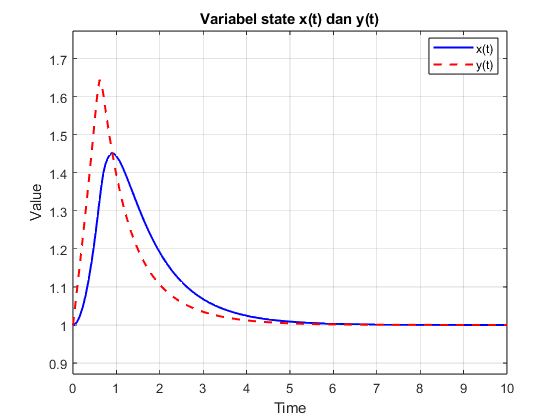
\includegraphics[width=0.45\linewidth]{EAS Nomor 2 x y.png}
    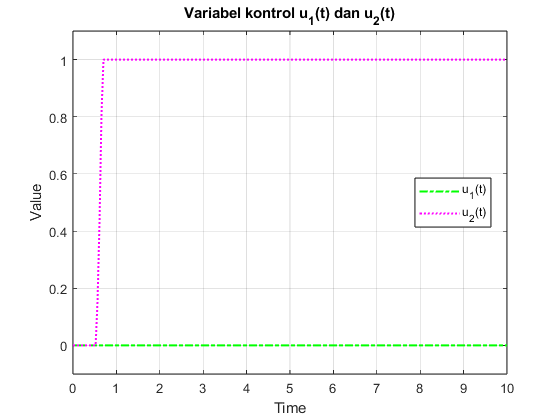
\includegraphics[width=0.45\linewidth]{EAS Nomor 2 u1 u2.png}
\end{figure}
    
\end{enumerate}

\end{document}
